
\documentclass[14pt]{extarticle}
\usepackage{fontspec}
\usepackage{polyglossia} % use instead of babel
\usepackage{pgfplots}
\usepackage{float}
\usepackage{amsmath}
\setdefaultlanguage{hebrew}
\setotherlanguage{english}
\newfontfamily\hebrewfont[Script=Hebrew]{Arial}

% TODO: figure out if better to keep this or not, for word document pdf output similarity
\usepackage[margin=1in]{geometry}

% might be useful to ensure similarity to word document pdf output
% \usepackage{setspace}
% \singlespacing

% Reset equation counter at the start of each section
\usepackage{chngcntr}
\usepackage{etoolbox}
\counterwithin*{equation}{section}
\preto{\section}{\setcounter{equation}{0}}

\begin{document}

\begin{center}
    {\LARGE \textbf{ממ"ן 16}}\\
    {\textbf{גלים במיתר}}
\end{center}

\begin{itemize}
    \item מגישים: תומר רוזנפלד, שי רואימי
    \item תאריך ביצוע הניסוי: 12 לאוגוסט 2025
    \item מדריך הניסוי: ד"ר סילביו ריינהורן
\end{itemize}
\newpage
\section*{ניסוי 1 - מהירות הגל במיתר מתוך מדידת תדרי התהודה בגל עומד}
\subsection*{מטרת הניסוי}
מציאת מהירות הגל במיתר על ידי מציאת תדרי התהודה שלו באורכי גל שונים.
\subsection*{רקע תיאורטי}
גל הוא הפרעה המתפשטת במרחב ונושאת אנרגיה. גלים מחזוריים מאופיינים ע"י תדירות $f$, אורך גל $\lambda$ ומהירות $v$. בין שלושת הגדלים מתקיים הקשר:
\begin{equation}
    v = \lambda \cdot f
\end{equation}

ע"פ החוק השני של ניוטון ניתן  להראות שקיים קשר בין מהירות  התפשטות הגל $v$ לבין מתיחות המיתר $T$ ו-\( \mu \) - צפיפות המסה הקווית של המיתר:
\begin{equation}
    \mu = \frac{m}{L}
\end{equation}
כאשר \(m\) הוא המסה של המיתר ו-\(L\) הוא אורכו. קשר זה הוא:
\begin{equation}
    v = \sqrt{\frac{T}{\mu}}
\end{equation}

גל עומד הוא הפרעה הנוצרת משילוב של שני גלים זהים הנעים בכיוונים מנוגדים ומתאבכים זה עם זה.
במצב זה שתי נקודות הקצה, נקודות המקסימום ונקודות המינימום קבועות במקומן.
נקודות המקסימום נקראות נקודות טבור, ורק גובהן משתנה עם הזמן, והנקודות בהן המיתר לא זז בכלל נקראות נקודות צומת. גל עומד מתקיים כאשר
\begin{equation}
    L=n*\frac{\lambda}{2}
\end{equation}

\subsection*{מערכת המדידה ומהלך הניסוי}
ראשית, בעזרת הנתונים במדריך הניסוי חישבנו את צפיפות המיתר הקווית. הצפיפות לא חושבה ע"י  מדידה ישירה כיוון  והמיתר קצר כך שמדידת  המשקל לא תהיה מדויקת

לאחר מכן חיברנו את המיתר למרטט מיתר  מצדו אחד, ומצדו השני  מעל לגלגלת חיברנו אליו משקולת של 150 גרם.
את  מרטט המיתר  חיברנו למחולל גל  סינוס.

לאחר מכן מצאנו את התדירות  בה מתקבל גל עומד, בעל אופן תנודה n=1,2,3,4,5. עבור כל מדידה נמדד גם כן  אורך הגל $\lambda$.

בעזרת המדידות, ושימוש בנוסחא (1) מצאנו את מהירות הגל במיתר, והשוונו אותה לתוצאה המתקבלת ע"י נוסחא (3).

לבסוף, כיוונו  את  תדר המחולל לערך בו לא מתקבל גל  עומד והקטנו את אורך  המיתר עד קבלת גל עומד.

\subsection*{תוצאות וניתוח}
ע"פ נוסחא (2), עבור $L=10m$, $m=3.14 grams$, נמצאה הצפיפות הקווית:
\begin{equation*}
    \mu = \frac{m}{L} = \frac{3.14 \cdot 10^{-3}}{10} = 3.14 \cdot 10^{-4} \frac{kg}{m}
\end{equation*}

מדידת המרחק ממרכז הגלגלת עד למרטט המיתר מצאה כי אורך המיתר:

$L=120cm$

לאחר מכן נמדדו התדירויות בהן מתקבל גל עומד עבור מספר מקטעים שונה:

\begin{table}[H]
    \centering
    \renewcommand{\arraystretch}{1.5} % Increase row height
    \begin{tabular}{|c|c|c|c|}
        \hline
        מספר מקטעים בגל עומד ($n$) & אורך הגל ($\lambda$) [$m$] & $\frac{1}{\lambda}$ [$\frac{1}{m}$] & תדירות המחולל ($f [Hz]$) \\
        \hline
        1                          & 2.4                        & 0.4167                              & 28.5                     \\
        2                          & 1.2                        & 0.8333                              & 57.4                     \\
        3                          & 0.8                        & 1.25                                & 85.6                     \\
        4                          & 0.6                        & 1.6667                              & 114.3                    \\
        5                          & 0.48                       & 2.0833                              & 142.2                    \\
        \hline
    \end{tabular}
    \caption{תאוצת העגלה בזוויות שונות}
\end{table}
את הנתנונים הללו ציירנו בגרף:

\begin{figure}[H]
    \centering
    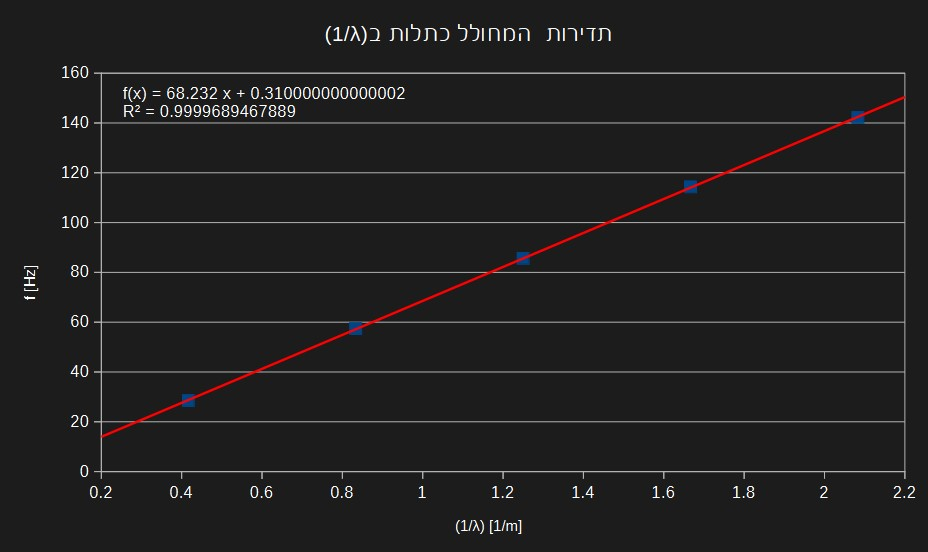
\includegraphics[width=0.8\textwidth]{frequency_to_1_over_lambda.jpg}
    \caption{גרף של תדירות הגל לעומת $\frac{1}{\lambda}$}
\end{figure}

מנוסחא (1), ע"י העברת אגפים ניתן  להסיק:
\begin{equation*}
    f = v\cdot \frac{1}{\lambda}
\end{equation*}
כלומר, שיפוע הגרף שווה למהירות הגל, ועל כן קיבלנו:

\begin{equation*}
    v = 68.232 \frac{m}{s}
\end{equation*}

חישוב אורך הגל בעזרת נוסחא (3) סיפק תוצאה קרובה:
\begin{equation*}
    v = \sqrt{\frac{T}{\mu}} = \sqrt{\frac{150 \cdot 10^{-3} \cdot 9.81}{3.14 \cdot 10^{-4}}} = 68.457 \frac{m}{s}
\end{equation*}

לבסוף, כיוונו את הערך המולל ל $70 [Hz]$, כך שלא מתקבל גל עומד. לאחר מכן הקטנו את אורך המיתר עד קבלת גל עומד עם שני מקטעים, האורך  שהתקבל הוא $L=0.98[m]$.
כאשר מתקבל גל עומד עם שני מקטעים ($n=2$), ואורך המיתר הוא $L=0.98[m]$, מתקיים:
\begin{equation*}
    \lambda = \frac{2L}{n} = \frac{2 \cdot 0.98}{2} = 0.98 \, m
\end{equation*}
ולכן ע"פ נוסחא (1):
\begin{equation*}
    v = f \cdot \lambda = 70 \cdot 0.98 = 68.6 \frac{m}{s}
\end{equation*}
כלומר, לא היה שינוי במהירות הגל.

\subsection*{דיון ומסקנות}
כאשר מצאנו את התדירות המאפשרת גל עומד בשני מקטעים ($f=54.7 [Hz]$), נשאלנו האם היחס $\frac{f2}{f1}$ תואם את התחזית שלנו.
נשים לב ליחס:
\begin{center}
    \begin{equation*}
        \begin{aligned}
            L = \frac{n \cdot \lambda}{2} \Rightarrow \lambda = \frac{2L}{n} \\ \\
            v=\lambda \cdot f \Rightarrow f = \frac{v}{\lambda} \Rightarrow f=\frac{v \cdot n}{2L}
        \end{aligned}
    \end{equation*}
\end{center}
ולכן  היחס בן התדירויות הוא:
\begin{equation*}
    \frac{f_2}{f_1} = \frac{v \cdot n_2}{2L} \cdot \frac{2L}{v \cdot n_1} = \frac{n_2}{n_1}
\end{equation*}
ובמקרה זה, $\frac{f_2}{f_1} = \frac{2}{1} = 2$, כלומר, התדירות הכפולה מתאימה למקטע כפול.
התוצאה שאנחנו קיבלנו היא: $\frac{f_2}{f_1} = \frac{57.4}{28.5} = 2.01$, קרוב מאוד לתוצאה התיאורטית. השגיאה היחסית  היא $\frac{|2.01-2|}{2} = 0.5\%$.

במהלך המדידות, כאשר נגענו בנקודת טבור אחת, הגל משתטח, ואם נגענו בנקודת צומת, לא קורה כלום. זאת כיוון ונקודת צומת אינה זזה, ולכן ההחזקה בה אינה משפיע על תנודת הגל.

לאחר מכן, נמדדה מהירות הגל בשני דרכים. האחת בעזרת התאמה ליניארית ונוסחא (1), שם התקבלה התוצאה: $v = 68.232 \frac{m}{s}$.
השנייה ע"י נוסחא (3), שם התקבלה התוצאה: $v = 68.457 \frac{m}{s}$.

השוואת התוצאות מראה כי הסטייה היחסית בין שתי השיטות היא:
\begin{equation*}
    \frac{|68.457 - 68.232|}{\frac{68.457 + 68.232}{2}} \cdot 100\% \approx 0.33\%
\end{equation*}

לבסוף, כיוונו את תדר המחולל לתדר $f=70[Hz]$ כך שלא נוצר גל עומד במיתר. הקטנו את אורך המיתר עד קבלת גל עומד עם שני מקטעים, והאורך שהתקבל הוא $L=0.98[m]$.

מהירות הגל כעת היא:
\begin{equation*}
    v = f \cdot \lambda = 70 \cdot 0.98 = 68.6 \frac{m}{s}
\end{equation*}

ניתן לראות שמהירות הגל לא השתנה, כלומר, היא נשמרה גם כאשר שינינו את אורך המיתר ואת תדר המחולל. מהירות הגל אינה תלויה באורך המיתר, כפי שראינו היא נתונה ע"י הנוסחא:
\begin{equation*}
    v=\sqrt{\frac{T}{\mu}}
\end{equation*}
כאשר $T$ הוא מתח המיתר, ו-$\mu$ היא צפיפות המסה הקווית של המיתר, שני גדלים שאינם תלויים באורך המיתר.

\section*{ניסוי 2 - צפיפות המיתר מתוך מדידת תדרי תהודה בגל עומד}
\subsection*{מטרת הניסוי}
מציאת צפיפות המיתר על ידי מדידת תדרי התהודה שלו במתיחיות שונות.
\subsection*{רקע תיאורטי}
בניסוי זה נעזר ביחס נוסף
\begin{center}
    \begin{equation*}
        \begin{aligned}
            T=mg \Rightarrow v = \sqrt{\frac{T}{\mu}} = \sqrt{\frac{mg}{\mu}} \Rightarrow v^2 = \frac{mg}{\mu} \\
            v=\lambda f \Rightarrow \lambda^2 f^2 = \frac{mg}{\mu} \Rightarrow f^2 = \frac{mg}{\mu \lambda^2}
        \end{aligned}
    \end{equation*}
\end{center}
ובהנתן גל עומד:
\begin{center}
    \begin{equation*}
        \begin{aligned}
            L=\frac{n \cdot \lambda}{2} \Rightarrow \lambda = \frac{2L}{n} \\
            f^2 = \frac{mg}{\mu \cdot (\frac{2L}{n})^2} = \frac{n^2 mg}{4 \mu L^2}
        \end{aligned}
    \end{equation*}
\end{center}
כלומר:
\begin{equation}
    f^2 = \frac{g}{\mu} (\frac{n}{2L})^2 \cdot m
\end{equation}

\subsection*{מערכת המדידה ומהלך הניסוי}
בניסוי זה מקמנו חיברנו את אותו החוט כמו בניסוי הקודם, מצד אחד למרטט ומצד שני לגלגלת כאשר בקצה החוט מחוברת משקולת של 50 גרם.

כיוונו את תדירות המחולל כך שהתקבל גל עומד בעל ארבעה מקטעים.

לאחר מכן, עבור מסות משקולות שונות, מצאנו את תדירות המחולל כך ששוב יווצר גל עומד בעל ארבעה מקטעים.

בעזרת תוצאות אלו, ושימוש בנוסחא (1), מצאנו את צפיפות המיתר.

\subsection*{תוצאות וניתוח}
תוצאות מדידת התדירויות עבורן התקבל גלמ עומד בעל ארבע מקטעים מתוארים בטבלה הבאה:

\begin{table}[H]
    \centering
    \renewcommand{\arraystretch}{1.5} % Increase row height
    \begin{tabular}{|c|c|c|}
        \hline
        מסה של המשקולת ($m [grams]$) & תדירות המחולל ($f [Hz]$) & $f^2 [Hz^2]$ \\
        \hline
        50                           & 66.2                     & 4382.44      \\
        100                          & 93.5                     & 8742.25      \\
        150                          & 114.3                    & 13064.49     \\
        200                          & 131.7                    & 17344.89     \\
        250                          & 145.2                    & 21083.04     \\
        \hline
    \end{tabular}
    \caption{תדירויות המחולל עבור מסות שונות}
\end{table}

התאמת קו מגמה:
\begin{figure}[H]
    \centering
    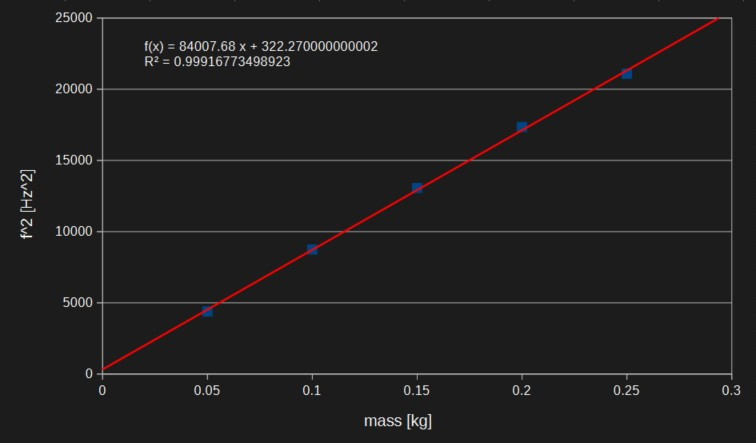
\includegraphics[width=0.7\textwidth]{frequency_squared_to_mass.jpg}
    \caption{קו מגמה עבור תדירויות המחולל}
\end{figure}

שיפוע הגרף שהתקבל הוא 84007.7. ע"פ נוסחא (1) נוכל למצוא את צפיפות המיתר:

\begin{center}
    \begin{equation*}
        \begin{aligned}
            f^2 = \frac{g}{\mu} (\frac{n}{2L})^2 \cdot m               \\
            \frac{g}{\mu} (\frac{n}{2L})^2 = 84007.7                   \\
            n=4, L=1.2[m], g=9.81[\frac{m}{s^2}]                       \\
            \mu = \frac{4^2 \cdot 9.81}{84007.7 \cdot (2 \cdot 1.2)^2} \\
            \mu = 3.244 * 10^{-4} [\frac{kg}{m}]
        \end{aligned}
    \end{equation*}
\end{center}
\subsection*{דיון ומסקנות}
בניסוי זה ראינו שקיים יחס ישר בין מסת המשקולות (המתח על המיתר) לבין $f^2$, ובעזרתו יכלנו למצוא  את צפיפות החוט.

הצפיפות הנתונה בניסוי הקודם הייתה $3.14 * 10^{-4} \frac{kg}{m}$

בניסוי זה מצאנו $\mu = 3.244 * 10^{-4} [\frac{kg}{m}]$. השגיאה היחסית היא:
\begin{equation*}
    \frac{|3.244 \cdot 10^{-4} - 3.14 \cdot 10^{-4}|}{3.14 \cdot 10^{-4}} \cdot 100\% \approx 3.3\%
\end{equation*}

\section*{ניסוי 3 - מדידות במיתר גמיש}
\subsection*{מטרת הניסוי}
מדידת מהירות הגל וצפיפות המיתר במיתר גמיש, בעזרת מדידת תדירות גלים עומדים.
\subsection*{רקע תיאורטי}
בניסוי זה נעזר בנוסחאות שצוינו בניסויים הקודמים, ונשים לב שהמיתר בניסוי זה גמיש ובעל צפיפות קווית שונה.
\subsection*{מערכת המדידה ומהלך הניסוי}
ראשית מדדנו את צפיפות המיתר הגמיש ע"פ הנתונים בניסוי.

לאחר מכן, כפי שנעשה בניסוי 1, מדדנו את התדירויות המאפשרות גל עומד במספר מקטעים שונה

ובעזרת התוצאות מצאנו את מהירות הגל, והשוונו אותה לצוצאה המתקבלת ע"י הנוסחא:
\begin{equation*}
    v= \sqrt{\frac{T}{\mu}}
\end{equation*}

לאחר מכן, חזרנו על שעשינו בניסוי 2 - מציאת צפיפות המיתר בעזרת היחס:
\begin{equation*}
    f^2 = \frac{g}{\mu} (\frac{n}{2L})^2 \cdot m
\end{equation*}

\subsection*{תוצאות וניתוח}
בהוראות הניסוי נתון כי למיתר גמיש באורך 5 מטרים, מסה של 21.27 גרם. מצאנו את צפיפות המיתר:
\begin{equation*}
    \mu = \frac{21.27 \cdot 10^{-3}}{5} = 4.254 \cdot 10^{-3} [\frac{kg}{m}]
\end{equation*}

כאשר תלויה בקצו של המיתר הגמיש משקולת של 150 גרם, מצאנו את התדירויות בהן מתקבל גל עומד:

\begin{table}[H]
    \centering
    \renewcommand{\arraystretch}{1.5} % Increase row height
    \begin{tabular}{|c|c|c|c|}
        \hline
        מספר מקטעים בגל עומד ($n$) & אורך הגל ($\lambda$) [$m$] & $\frac{1}{\lambda}$ [$\frac{1}{m}$] & תדירות המחולל ($f [Hz]$) \\
        \hline
        1                          & 2.4                        & 0.4167                              & 7.8                      \\
        2                          & 1.2                        & 0.8333                              & 15.8                     \\
        3                          & 0.8                        & 1.25                                & 23.6                     \\
        4                          & 0.6                        & 1.6667                              & 31.7                     \\
        5                          & 0.48                       & 2.0833                              & 39.6                     \\
        \hline
    \end{tabular}
    \caption{תאוצת העגלה בזוויות שונות}
\end{table}

את הנתנונים הללו ציירנו בגרף:

\begin{figure}[H]
    \centering
    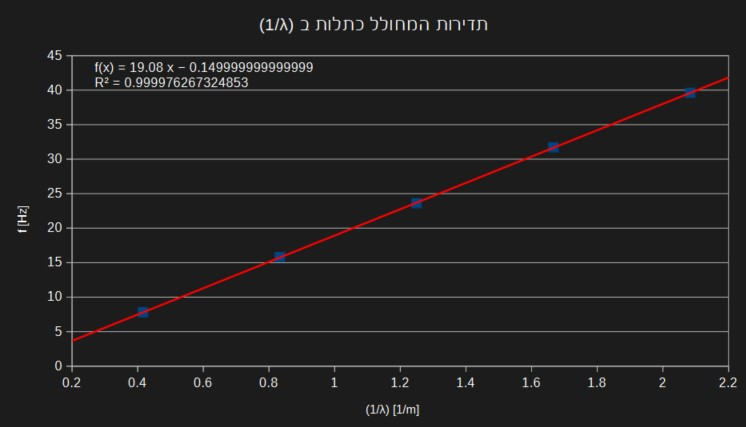
\includegraphics[width=0.8\textwidth]{stretchy_frequency_to_1_over_lambda.jpg}
    \caption{גרף של תדירות הגל לעומת $\frac{1}{\lambda}$}
\end{figure}

ע"פ ההתאמה הליניארית בגרף, השיפוע שהתקבל הוא  19.08, כלומר מהירות הגל היא:
\begin{equation*}
    v = 19.08 [\frac{m}{s}]
\end{equation*}

לאחר מכן חישבנו את מהירות הגל בעזרת הנוסחא: $v= \sqrt{\frac{T}{\mu}}$

נציב:
\begin{equation*}
    v= \sqrt{\frac{150 \cdot 10^{-3} \cdot 9.81}{4.254 \cdot 10^{-3}}} = 18.6 [\frac{m}{s}]
\end{equation*}

נשווה את התוצאות ונמצא סטייה יחסית:

\begin{equation*}
    \frac{19.08 - 18.6}{\frac{19.08 + 18.6}{2}} \cdot 100\% \approx 2.58\%
\end{equation*}

לאחר מכן ביצענו את ניסוי 2 עם המיתר הגמיש. מדדנו אילו תדירויות מאפשרות גל עומד בעל 4 מקטעים, עבור מתיחיות שונות:

\begin{table}[H]
    \centering
    \renewcommand{\arraystretch}{1.5} % Increase row height
    \begin{tabular}{|c|c|c|}
        \hline
        מסת המשקולת [kg] & תדירות המחולל [$Hz$] & $f^2$ [$Hz^2$] \\
        \hline
        0.05             & 18.5                 & 342.25         \\
        0.1              & 25.7                 & 660.49         \\
        0.15             & 31.7                 & 1004.89        \\
        0.2              & 37                   & 1369           \\
        0.25             & 41.8                 & 1747.24        \\
        0.3              & 48.1                 & 2313.61        \\
        0.35             & 54.5                 & 2970.25        \\
        \hline
    \end{tabular}
    \caption{תדירויות ומהירויות עבור מתיחויות שונות}
\end{table}

את הנתנונים הללו ציירנו בגרף:

\begin{figure}[H]
    \centering
    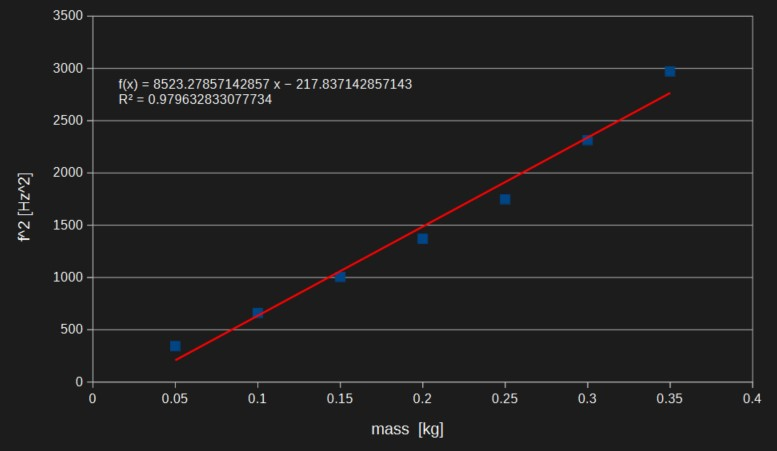
\includegraphics[width=0.7\textwidth]{stretchy_frequency_squared_to_mass.jpg}
    \caption{קו מגמה עבור תדירויות המחולל}
\end{figure}

ניתן לראות שאין התאמה ליניארית טובה ($R^2=0.976$). את הסיבה לכך אסביר בחלק הבא.

כעת נצייר גרף לפי 4 הנקודות הראשונות בלבד:

\begin{figure}[H]
    \centering
    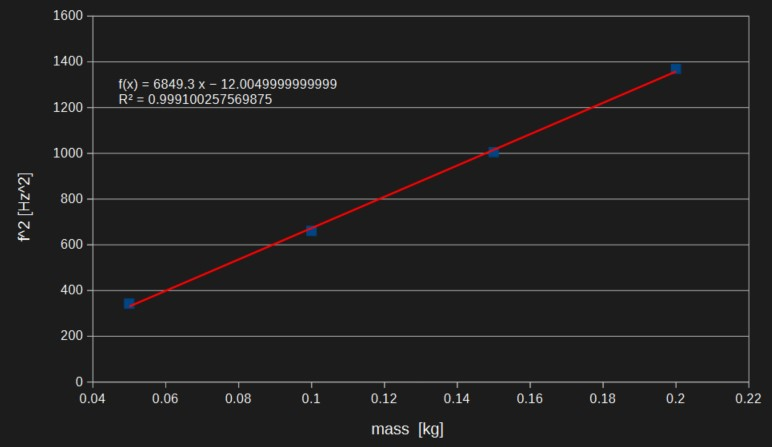
\includegraphics[width=0.7\textwidth]{stretchy_frequency_squared_to_mass_first_4_points.jpg}
    \caption{קו מגמה עבור תדירויות המחולל}
\end{figure}

ניתן לראות כעת שההתאמה הליניארית יותר טובה. נמצא את צפיפות המיתר כפי שעשינו בניסוי 2.

שיפוע הגרף שהתקבל הוא 6849.3:

\begin{center}
    \begin{equation*}
        \begin{aligned}
            f^2 = \frac{g}{\mu} (\frac{n}{2L})^2 \cdot m               \\
            \frac{g}{\mu} (\frac{n}{2L})^2 = 6849.3                   \\
            n=4, L=1.2[m], g=9.81[\frac{m}{s^2}]                       \\
            \mu = \frac{4^2 \cdot 9.81}{6849.3 \cdot (2 \cdot 1.2)^2} \\
            \mu = 3.978 * 10^{-3} [\frac{kg}{m}]
        \end{aligned}
    \end{equation*}
\end{center}

השגיאה היחסית ביחס למדידה בסעיף 1 היא:
\begin{equation*}
\frac{|3.978 * 10^{-3} - 4.254 * 10^{-3}|}{4.254 * 10^{-3}} \cdot 100\% \approx 6.48\%
\end{equation*}

\subsection*{דיון ומסקנות}
בניסוי זה ביצענו את ניסויים 1 ו-2 עם מיתר גמיש.

תחילה מדדנו את התדירות הנדרשת ליצירת  גל עומד עם מספר מקטעים שונים, ולאחר מכן בדקנו אילו תדירויות נדרשות על מנת לייצר גל עומד עם ארבעה מקטעים, כאשר מחובר משקל שונה לחוט כל פעם.

בחישוב מהירות הגל, הסטייה היחסית בין שתי השיטות בניסוי הראשון הייתה $0.33\%$ ובניסוי הזה הסטייה היחסית הייתה $2.58\%$.

וכן בחישוב הצפיפות, בניסוי השני הסטייה היחסית הייתה $3.3\%$ ובניסוי הזה הסטייה היחסית הייתה $6.48\%$.

בניסוי זה המיתר היה גמיש, וזה המקור לסטיות הגבוהות יותר. בתיאוריה מניחים כי אורך החוט קבוע, ולכן הצפיפות הקווית $\mu=\frac{m}{L}$ נשארת קבועה ללא תלות במתח. בפועל המיתר הגמיש נמתח כתוצאה מהמסות התלויות ואורכו $L$ גדל.

כתוצאה מכך, הצפיפות הקווית $\mu$ קטנה, וזה משפיע על מהירות הגל המחושבת לפי $v=\sqrt{\frac{T}{\mu}}$.

סיבה זו היא הגורם לחוסר ההתאמה הליניארית בגרף (איור 4). באיור 5 ציירנו גרף של ארבע הנקודות הראשונות בלבד, בהן המשקל התלוי היה הנמוך ביותר, כתוצאה מכך המיתר נמתח פחות והתוצאה שהתקבלה הייתה יותר קרובה לחישוב שנעשה בתחילת הניסוי.

לסיכום, מהירות הגל במיתר נקבעת ע"י מתיחות המיתר $T$ ועל ידי הצפיפות הקווית שלו $\mu$. אורך המיתר, אופן התנודה ותדירות אינם משפיעים ישירות על מהירות הגל, אבל קובעים את התנאים להיווצרות גל עומד.

\section*{שאלה בונוס}
התבקשנו להוכיח את נוסחא (3) ברקע התיאורטי:
\begin{equation*}
L=n\frac{\lambda}{2}
\end{equation*}

\end{document}